\chapter{Theoretical Background}
\label{theoretical_background}
This chapter will cover the needed theoretical background to understand the working principle of the Artificial Eye. 

\section{Light}
Electromagnetic radiation can be classified by its wavelength $\lambda$ or frequency $f$ as shown in figure \ref{ElectromagneticSpectrum}. Light is defined as a small part of the electromagnetic spectrum which makes vision possible for the human eye. The healthy human eye can detect electromagnetic radiation in a range starting at 360 - 400nm (blue light) up to 760 - 830nm (red light). Infrared and ultraviolet radiation are not visible for the human eye but are often included into the category of light and are referred to as "Infrared light" and "Ultraviolet light".\cite{NoboruOhta2005}


\begin{figure}
\begin{center}
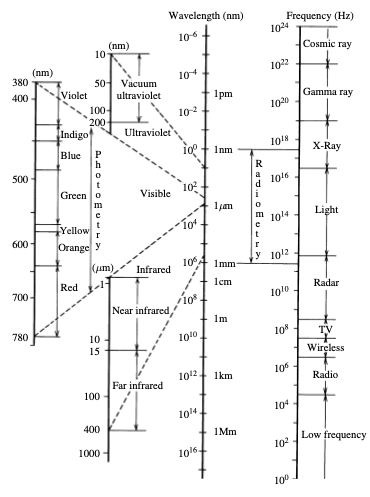
\includegraphics[width=12cm]{Pictures/ElectromagneticSpectrum}
\caption[Wavelength of the electromagnetic radiation and light]{Wavelength of the electromagnetic radiation and light\cite{NoboruOhta2005}}
\label{ElectromagneticSpectrum}
\end{center}
\end{figure}


\subsection{Polarisation of Light}
The polarisation of light is a property which the human eye cannot sense. Polarisation of electromagnetic waves is based on the phenomena that the wave is oscillating perpendicular to its axis of motion. Polarisation can be either linear, right hand circular/elliptical or left hand circular/elliptical polarised. The orientation of the polarisation is described by the orientation of the plane in which the wave oscillates. For linear polarised light, the orientation of this plane is constant. For circular or elliptical polarised light, the plane of oscillation is rotating around the direction of movement of the wave. The three different states of polarisation are shown in figure \ref{Polarisation}.\\
Similar to the human eye, it exists no meteorological usable effect to measure the polarisation of light directly. Only with the intelligent use of polarising optics, the polarisation of light can be transferred into a measurable intensity.\cite{LoefflerLang2020}\cite{hecht2002optics}\\
The property of polarisation in practical applications is often used to distinguish between different light signals. For example in light curtains: A light curtain consists of a sender and a receiver. The sender transmits a beam of polarised light towards the receiver. The receiver then measures the intensity of the incoming light and signals when it drops below a certain threshold. This drop in light intensity can be caused for example by an object blocking the path between transmitter and receiver. To determine whether the measured intensity is the light transmitted by the transmitter of the light curtain or environmental noise, the receiver filters the light for the polarisation direction of the light beam coming from the transmitter. This is highly effective, because environmental noise caused by lamps or sunlight is unpolarised in most cases (randomly polarised) light and has therefore only a very small intensity in the polarisation detection range of the light curtain receiver.\cite{LoefflerLang2020}\cite{PilzLightBarrier}

\begin{figure}
\begin{center}
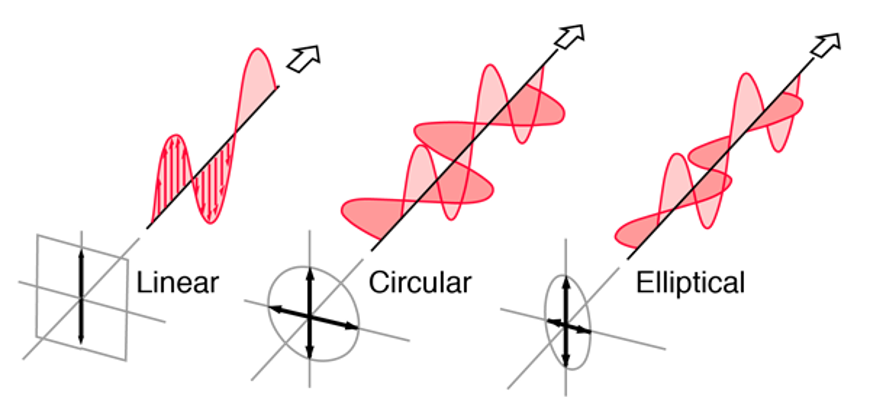
\includegraphics[width=12cm]{Pictures/Polarisation}
\caption[Different states of polarisation]{Different states of polarisation\cite{GSUPolarization}}
\label{Polarisation}
\end{center}
\end{figure}







\section{Optical systems and components}
Optical systems can consist of a multitude of lenses and other devices but can also be as simple as the famous "Camera obscura" which only consists of a hole (aperture) and a screen for imaging.

\subsection{Lenses}
Lenses are a refracting, transparent and often spherical devices used in optics. They either focus or disperse and can, based on this property, be divided into two main groups: converging and diverging. Lenses are characterised by their focal length $f$. The focal length describes the distance between the principal plane of the lens and its focal point. The focal point (F) describes the point where the incoming light beam is focussed on after passing through the lens and its focal point F. Figure \ref{Lens} shows the path of light for both, a converging lens and a diverging lens. Converging lenses have a focal length greater than zero ($f>0$) and diverging lenses have a focal length smaller than zero ($f<0$), the focus point is located in front of the lens.\cite{LoefflerLang2020}\\
Because spherical lenses are easy and cheap to manufacture, they are one of the most used type of lens. With the advancing manufacturing and measuring technologies, aspherical lenses (the surface of an aspherical lens is not longer a section of a sphere) are used more and more. Aspherical lenses have an improved imaging quality. Image distortions, so called "optical aberrations" can be completely eliminated using aspherical lenses.\\
To improve image resolution and colour quality, modern lenses for photography or machine vision tasks contain many different smaller lenses. Further, they often feature additional functions like zoom (adjustable focal length) and an adjustable aperture to control the amount of light which is entering the camera system.\cite{LoefflerLang2020}\cite{ThorlabsMachineVisionLenses}

\begin{figure}
\begin{center}
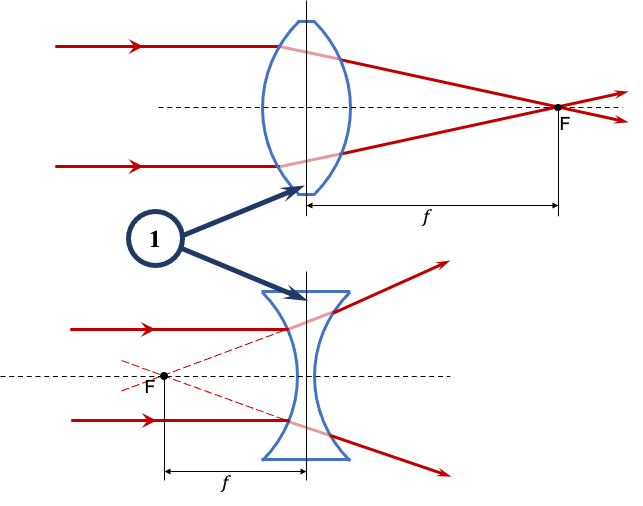
\includegraphics[width=12cm]{Pictures/Lenses}
\caption[Drawing of path of light for a spherical converging and diverging lens]{Drawing of path of light for a spherical converging and diverging lens: Top - Converging lens, Bottom - Diverging lens, 1 - Principal plane of the lens}
\label{Lens}
\end{center}
\end{figure}

\subsection{Beamsplitter}
A beamsplitter is an optical device which splits an incoming light beam into two or combines two light beams into one. Beamsplitters are usually made by applying a thin partial reflective or Beam splitting (BS) coating to one side of a prism and gluing it to another one. This is shown in \ref{beamsplitter_shematic}. In the most common type of beamsplitter the rate between transmission and reflection is 50/50. Beamsplitter can be both, polarising and non-polarising. Non polarising beamsplitter will not effect the polarisation of the incoming light. For polarising beamsplitter the transmission and reflection of the light is dependant on the polarisation direction of the incoming light.\cite{ColourApperance}

\begin{figure}
\begin{center}
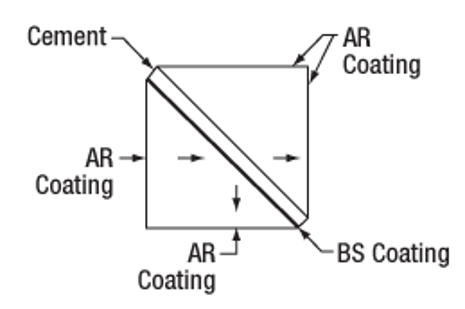
\includegraphics[width=12cm]{Pictures/Beamsplitter}
\caption[Schematic of a non-polarising beamsplitter]{Schematic of a non-polarising beamsplitter\cite{ThorlabsBeamsplitter}: AR - Anti Reflective Coating, BS - Beam Splitting Coating}
\label{beamsplitter_shematic}
\end{center}
\end{figure}

\subsection{Optical Filter}
Optical filters precisely absorb or reflect radiation in certain wavelengths, while transmitting others. They are used to select a specific band of wavelengths, intensity or polarisation within an optical system. Optical filters are widely used in areas like photography, microscopy, spectroscopy or machine vision and can simply consist of coloured glass.\cite{IDEXFilterSelection}\cite{LoefflerLang2020}

\subsubsection{Edge-pass Filter}
Edge-pass filters start or stop transmitting light at a specific wavelength abruptly. These types of filters are typically divided into "Long-pass" and "Short-pass" filters. Long-pass filters transmit light with a wavelength longer then the "Cut-On" wavelength of the optical filter. Short-pass filters on the other hand only transmit light with a wavelength shorter than their "Cut-Off" wavelength. Figure \ref{longpass_diagram} shows a typical transmission curve for an edge-pass filter.  

\begin{figure}
\begin{center}
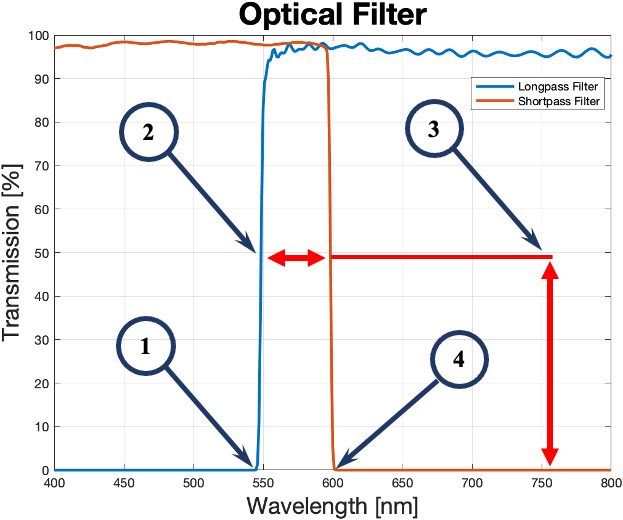
\includegraphics[width=12cm]{Pictures/Longpass.png}
\caption[Diagram of two Edge-pass filter, combined to an Bandpass-filter with a FWHM of 50nm]{Diagram of two Edge-pass filter, combined to an Bandpass-filter with a FWHM of 50nm\cite{ThorlabsEdgepass} : 1 - Cut On Frequency, 2 - Full Width at Half Maximum, 3 - Half Maximum, 4 - Cut Off Frequency}
\label{longpass_diagram}
\end{center}
\end{figure}

\subsubsection{Bandpass Filter}
Optical bandpass filters transmit a specific band of wavelengths. The transmission band of such a filter is described by the term "Full width at half maximum" (FWHM) around a specific "Center Wave Length" (CWL). The CWL describes the middle of the transmission band, while the term FWHM is used to describe the width of the transmission band at half of the maximum transmission rate. The width of the transmission band can be as small as 1 nm or as wide as hundreds of nanometers. Bandpass filters can be purchased as such, but can also be created by combining long-pass and short-pass filters. This is shown in figure \ref{longpass_diagram}.

\subsubsection{Polariser}
A polariser or polarisation filter is an optical device which selects light with a specific state of polarisation, while blocking all others. Polarisers can select one specific polarisation out of a beam of randomly polarised light and turn it into a beam of light with a defined polarisation state. However, it is important to notice, that a polariser cannot influence the state of polarisation of light but only select an existing one.\cite{hecht2002optics}

\subsection{Optical retarder}
An optical retarder or "Wave-plate" is a component used in optics which alters the polarisation state of light travelling through it. The most common types of wave-plates are the "half wave-plate", which turns the polarisation plane of polarised light, and the "quarter wave-plate" which can convert linear polarised light into circularly or elliptical polarised light and vice versa.\\
A wave-plate has two principal axes. These axes are perpendicular to each other and are usually referred to as "fast" and "slow" axis. Is the polarisation of the light aligned with the fast axis of the wave-plate, it will not be affected. When aligned with the slow axis of the wave-plate it will be delayed by quarter of its wavelength (a quarter wavelength when using a quarter wave-plate and a half wavelength when using a half wave-plate). Is the polarisation not aligned with one of the two axes, it can be considered a split into two parts. One aligned with the fast axis, one aligned with the slow axis. The resulting polarisation state of the light is the sum of both parts (the un-delayed part and the delayed part) after passing through the wave-plate. In optical applications, wave-plates are often used in combination with a polariser to turn randomly polarised light into circular polarised light. This effect is for example used in cinemas to create 3-D images.\cite{LoefflerLang2020}\cite{hecht2002optics}\cite{MITHalfWP}\cite{MITQuarterWP}


\subsection{Digital Cameras}
A digital camera is an optoelectronic device which captures a picture and saves it as digital information to a digital memory. Most digital cameras have a similar setup and are used in combination with an optical system in form of a machine vision or photographic camera lens. Similar to the human eye, the lens system is used to adjust the focus of the camera system as well as the amount of light which is passed to the image sensor. The image sensor is constructed as an array of light sensible electronics so called "Electro-optical transducer". Depending on if the camera system is supposed to capture a coloured or monochromatic image, a filter pattern is applied to the sensor array. One of the most used filter patterns is the "Bayer Pattern". The Bayer Pattern is shown in figure \ref{BayerPattern}. It consists of filters for the three primary colours red, green and blue (2x2 pixel pattern with double green filter). The intensity of the colour-filtered light can then in post processing be combined into a coloured picture.\cite{LoefflerLang2020} 

\begin{figure}
\begin{center}
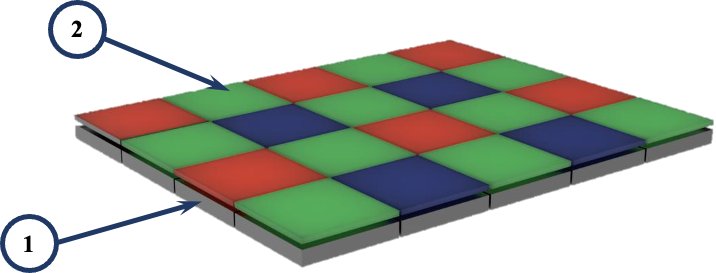
\includegraphics[width=12cm]{Pictures/BayerPattern}
\caption[Picture of the Bayer Pattern]{Picture of the Bayer Pattern: 1 - Semiconductor Pixel, 2 - Bayer Filter Pattern}
\label{BayerPattern}
\end{center}
\end{figure}

Depending on the requirements, the individual optics and electronics of digital cameras can be very different. For example, while a photography camera is built to capture high resolution images with a good colour representation, a machine vision camera is eventually built to process and transfer captured images with least amount of latency to an analysis system. An important choice at this point is the type of image sensor that is used to convert the light signal into an electrical one. The two most common types of image sensors for visible light are the Charge Coupled Device (CCD) and the Complementary Metal Oxide Semiconductor (CMOS) image sensor:

\subsubsection{CCD Image Sensor}
A CCD image sensor consists of a number of light sensitive semiconductor sensor elements, called pixels. These elements can either be assembled as a row or a matrix. The CCD elements absorb the incoming photons and build up an electrical charge, which is proportional to the intensity of the photons. The efficiency (electrical charge/incoming photons) of CCD elements is very good ($\sim$1). This and their resistance against environmental interference makes them a good choice for critical applications with less light such as astronomy. The physical size of one CCD pixel is usually 2 to 30 $\mu$m. The electronics for collecting, amplifying and processing the charge signal is in contrast to CMOS chip not integrated into the CCD and needs to be done by external. Caused by an electronic interference called capacitive coupling, the charge value of the pixel cannot be transferred to the amplifying electronics instantly. Instead the external electronics need to push the charges into a so called "Shift Register". This is done by applying an external voltage across every pixel. Once the charge value of each pixel is saved in the shift register, they can be pushed (shifted) out one by one to be processed by the image processing electronics.\cite{LoefflerLang2020}

\begin{figure}
\begin{center}
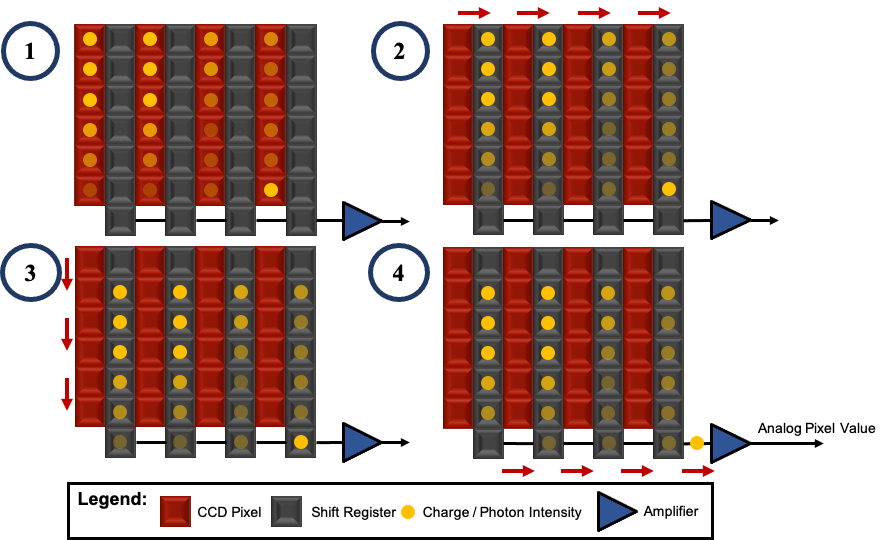
\includegraphics[width=12cm]{Pictures/CCDShifting}
\caption[Scheme of the image acquisition process using a CCD sensor]{Scheme of the image acquisition process using a CCD sensor: 1 - The CCD pixels are exposed to light, 2 - The collected charge values are shifted into the Shift Register, 3 - The charge values are shifted down row by row, 4 - Each row is shifted into the Amplifying Circuit pixel by pixel}
\label{CCDShifting}
\end{center}
\end{figure}

\subsubsection{CMOS Image Sensor}
CMOS image sensors are similarly to CCD sensors based on small semiconductor pixels to translate the intensity of incoming photons into an electric signal. In contrast to the CCD image sensor, each CMOS pixel has the electronics for the signal amplification and transfer built into the silicon chip. This eliminates the problematic with capacitive coupling and provides an already amplified voltage signal to the processing electronics. To be able to read the voltage signal of each pixel conveniently, they are often connected in form of a logical grid with rows and columns. This way each pixel can be addressed separately. The processing electronics then read the image data row by row and pixel by pixel. The disadvantage of this type of image acquisition is an effect called "rolling shutter". Because the value of each pixel is acquired separately, the time needed to read and process the pixel data a time delay accumulates during the reading process. This can be visible when imaging fast moving objects. Caused by the delay between reading the first and the last pixel, the motion of the object will be visible in the resulting picture. This problem can be solved with a so called "global shutter". A global shutter exposes every pixel to the incoming light at the same time. This is done by pushing the values of all pixels into a fast temporary memory, similar to the CCD sensor.\cite{LoefflerLang2020}\cite{Basler2018RollingShutter} 

\subsection{Optical Spectrometer}
An optical spectrometer (often referred to as spectrograph or spectrophotometer), is an optical device used to measure the properties of an electromagnetic spectrum. The measured property can either be intensity/wavelength or polarisation/wavelength. The measurement principle of a spectrometer is based on a monochromator setup. A well known monochromator setup is the "Czerny-Turner monochromator". As shown in figure \ref{CzernyTurnerSpec}, the light enters the monochromator through a small entry slit. Next, a mirror collimates the light beam and reflects it towards a diffraction grating. The diffraction grating splits the light into its spectral components. Finally, another mirror focuses the light beam onto a CCD array for quantification of the spectrum.\cite{LoefflerLang2020}\\
A spectrometer can be used for a variety of different tasks. The three most common ones are the examination of a light source, the measurement of the reflective properties of a surface (spectrophotometer used for colour measurements) and the absorption properties of a liquid.

\begin{figure}
\begin{center}
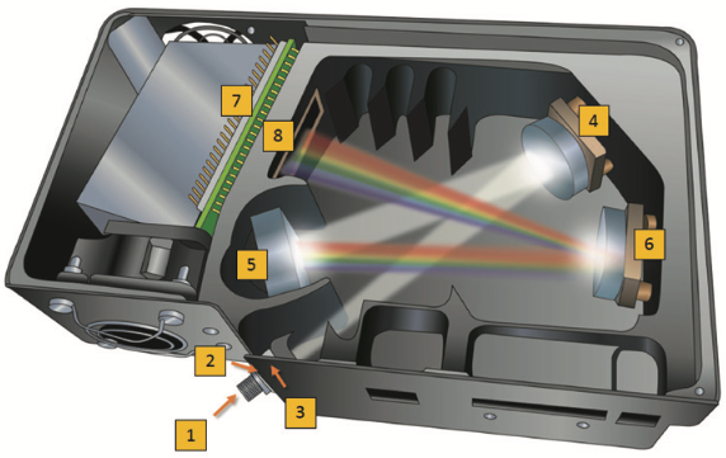
\includegraphics[width=12cm]{Pictures/CzernyTurnerSpect}
\caption[Graphic of a spectrometer with a Czerny-Turner monochromator]{Graphic of a spectrometer with a Czerny-Turner monochromator\cite{LoefflerLang2020}: 1 - Connector for optical fibre, 2 - Endstop for fibre connector, 3 - Entry slit, 4 - Collimating mirror, 5 - Diffraction grating, 6 - Focusing mirror, 7 - Electronics, 8 - CCD Array}
\label{CzernyTurnerSpec}
\end{center}
\end{figure}






\section{Mechanical systems}

\subsection{Translation stages}
A translation stage or linear stage is a mechanical device, which can move only along one axis. Therefore its Degree of Freedom (DoF) is one. Translation stages usually consist of a rigid body and a slide. The setup of a translation stage is shown in figure \ref{LinearStage}. The body of the stage can be fixed to an optical table or any other fixture. The slide can move relative to the body along one axis. To restrict the movement of the slide to a linear movement along one axis only, it is placed on precision ground linear rails. The linear stage can be operated manually or driven by an electric motor via a ball screw, which is attached to the slide. Electrical actuated linear stages can reach a positional accuracy of op to 2 $\mu$m with a repeatability of 1 $\mu$m \cite{Thorlabs2018LinStage}.\\
Translation stages are used in optics to precisely move optical components relative to each other or to an object of interest. For example to focus a camera system onto a stationary object.\cite{LoefflerLang2020}

\begin{figure}
\begin{center}
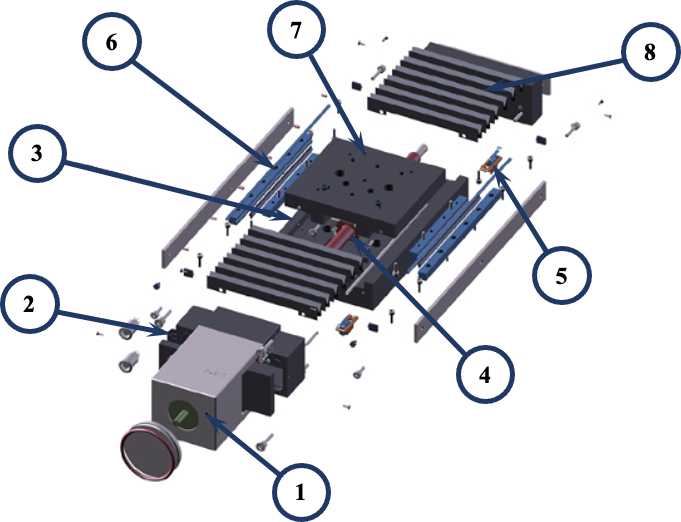
\includegraphics[width=12cm]{Pictures/LinearStage}
\caption[Exploded-view drawing of a translation stage]{Exploded-view drawing of a translation stage\cite{LoefflerLang2020}: 1 - Stepper-motor,  2 - Control Electronics, 3 - Body, 4 - Ball screw, 5 - End switch for zero point reference, 6 - Linear rails, 7 - Slide, 8 - Way covers}
\label{LinearStage}
\end{center}
\end{figure}

\subsection{Cartesian motion system}
A cartesian motion system is used to move an endeffector or part in two or more axes. Depending on the desired Degree of Freedom it is built from two to three linear axes and up to three rotational axes. Similar to a cartesian coordinate system all translation and rotation axes are perpendicular to each other. This way, each motion axis can move independently from the other axes in one cartesian coordinate. The cartesian motion system is probably the most intuitive and most used motion system. It can be found in a wide variety of CNC and robotics applications, such as: CNC-Mills, 3D-Printers and Pick \& Place Machines.\cite{Mareczek2020}


\section{Soft Metrology}
Soft metrology is the science that covers the development of measurement methods and mathematical models used to objectively describe properties of materials or products which are determined by the human perception. A good example for the use of the methodology of soft metrology shows the design process of a product which is intended to interact with any of the five senses (sight, sound, smell, taste and touch). Here the designers want to predict the subjective human perception and quantify it on an objective scale in order to guarantee a flawless user experience with the product.\cite{Eugene2008}

\subsection{The Human Eye}
Similar to a modern digital camera, the human eye is a sink for electro magnetic radiation. In combination with the human brain it features a complex optical imaging and image processing system. In the human eye, light enters through the cornea. The cornea works, together with the aqueous humour (a fluid encapsulated behind the cornea), as a lens which bends the light towards the iris. The iris is a ring-shaped muscle behind the cornea and the aqueous humour. It controls the amount of light entering the eye by widening or narrowing the diameter of the entry hole similar to the aperture in a camera lens. Next, the light needs to pass through the lens of the human eye. This lens is a clear flexible disc, attached to small muscles. These muscles can deform the lens and represent the "autofocus" system of the human eye focussing the light onto the retina. The retina is located in the back of the eye and is quantifying the spectrum of the incoming light and its intensity. In figure \ref{HumanEye} a cross-section of the human eye is shown.\cite{Frings2019}\cite{LoefflerLang2020}\\
The retina is the light sensing part of the human eye and consists of approximately 126 million photoreceptors. These photoreceptors are divided in "Rods" and "Cones" and are responsible to convert the incoming electromagnetic signal into an electrical signal which can be processed by the cortex. These two types of photoreceptors are very different in their functionality. Rods are highly sensible in a wide range of wavelengths and are responsible to give sight at night or in bad lighting conditions. However, Rods cannot resolve colours. Colour vision is provided by the signals coming from the Cones on the retina. The Cones are split into three different types: L-Cones, M-Cones and S-Cones. Each of them sensible for a different band of wavelengths and therefore a different colour, as indicated by the letters L, M and S (Long, Medium and Short wavelength cone). These "biological bandpass filters" provide the colour signal red, green and blue which is then processed into a coloured image by the brain.\cite{SensationandPerception}\cite{Frings2019}


\begin{figure}
\begin{center}
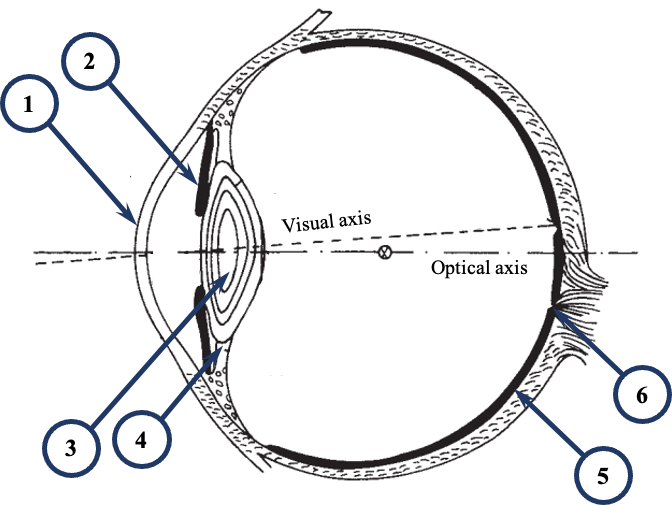
\includegraphics[width=12cm]{Pictures/HumanEye}
\caption[Cross section of the human eye]{Cross section of the human eye\cite{LoefflerLang2020}: 1 - Cornea, 2 - Iris, 3 - Lens, 4 - Ciliary Muscle, 5 - Retina, 6 - Connection point of the Optical Nerve}
\label{HumanEye}
\end{center}
\end{figure}

\subsection{The human visual perception}
Being a very complex topic, a wide variety of theories about the human visual perception exists. A widely known and probably the most accepted theory is the "opponent process theory". It explains the human colour perception based on the combination of the colour signals coming from the photoreceptors in the human eye. The theory explains the perception of white as the state where the three different types of cones (L + M + S) are maximal excited. In contrast to this, the human vision system perceives something as black, when the three types of cones are maximal inhibited. The same principle applies to the perception of Red \& Green as well as Blue \& Yellow.\cite{Wolfe1957} However, the perception of colour can be altered by the contrast of different coloured surfaces nearby. In fact, the visual system interprets colours of surfaces close together by comparing the intensity of the reflected light from one to another.\cite{Chanal2020}\cite{Gilchrist1979}

\subsection{Colorimetry}
Colorimetry is a scientific approach of measuring and describing the human colour perception. This is not an easy task, because human perception is often very subjective and dependant on a lot of variables as for example: the lighting situation, surface texture or contrast. For this reason the definition of colour is split into two parts: perceived colour and colour stimulus, the latter often referred to as "true colour".\\
The measuring of colours is based on the phenomena that materials interact differently with certain portions of the electromagnetic spectrum. In the simplest case a material either reflects a certain wavelength or absorbs it. The sum of the visible electromagnetic spectrum reflected by a surface is what the human eye and brain perceives as colour. Colour measurement devices, for example so called spectrophotometers, use this by shining a well defined spectrum of light onto a surface and comparing it to the spectrum of light which is reflected back. This resulting spectrum of light can then be transferred into a so called "Colour space". The probably most widely known colour space is the RGB colour space. RGB describes colours by mixing its three primary colours red, green and blue additively. The connection between the RGB colour space is made by the CIE 1931 colour space which describes the light spectrum for the three primary colours of RGB. The CIE 1931 colour space and the definition of the RGB primaries are shown in figure \ref{CIE}.

\begin{figure}
\begin{center}
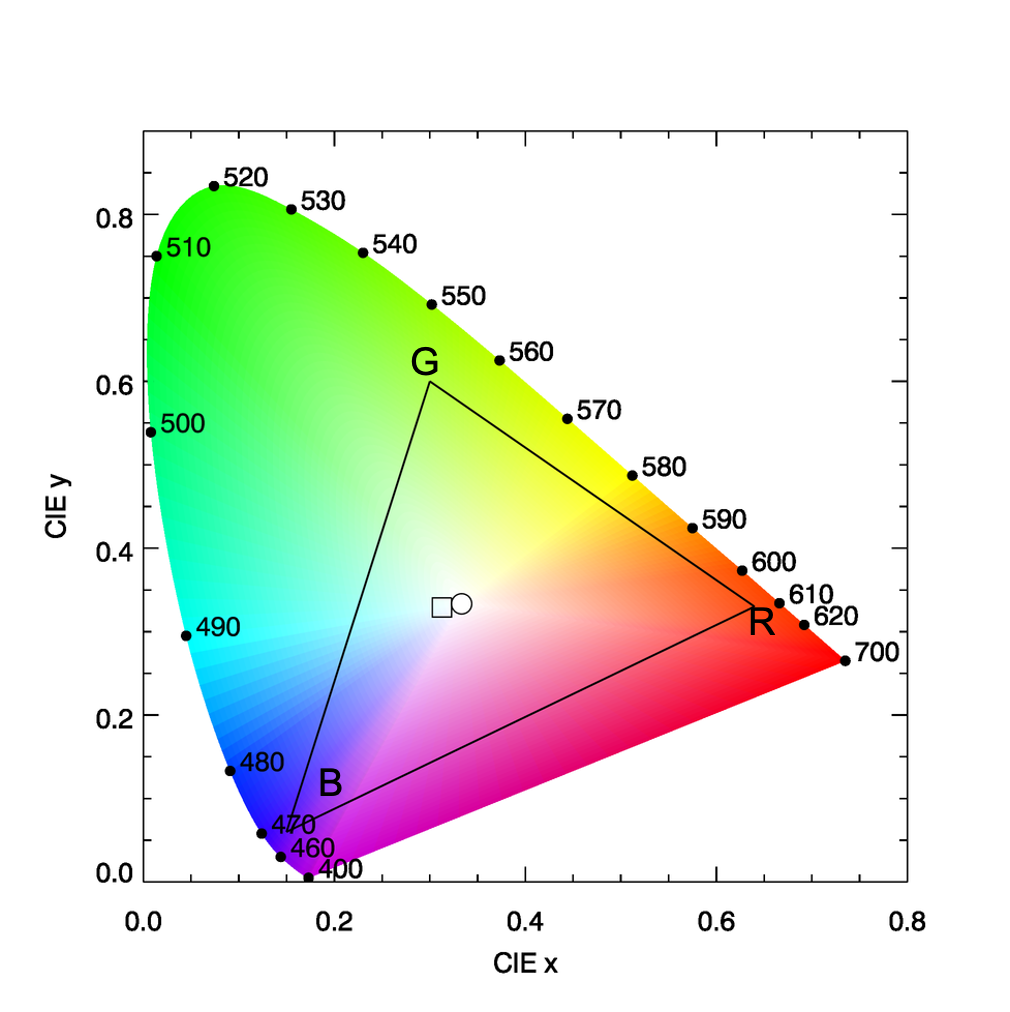
\includegraphics[width=12cm]{Pictures/CIEColour}
\caption[Illustration of the RGB definition in the CIE 1931 colour space]{Illustration of the RGB definition in the CIE 1931 colour space\cite{OceanOpticsCIE}}
\label{CIE}
\end{center}
\end{figure}






\section{Hard Metrology}
While soft metrology focuses on methods and models to objectively describe the subjective human perception of materials or products, hard metrology focuses on methods to take discrete, objective measurements of samples.

\subsection{Surface Metrology}
There are many very different methods to determine the topography of a surface but the most common can be (see figure \ref{TopologyMM}) divided into contacting and contact-free. Contacting topography measurement methods are often also called mechanical methods, due to their mechanical interaction with the surface of the sample. In contrast to that contact-free measurement methods can be divided into optical or acoustic.

\begin{figure}
\begin{center}
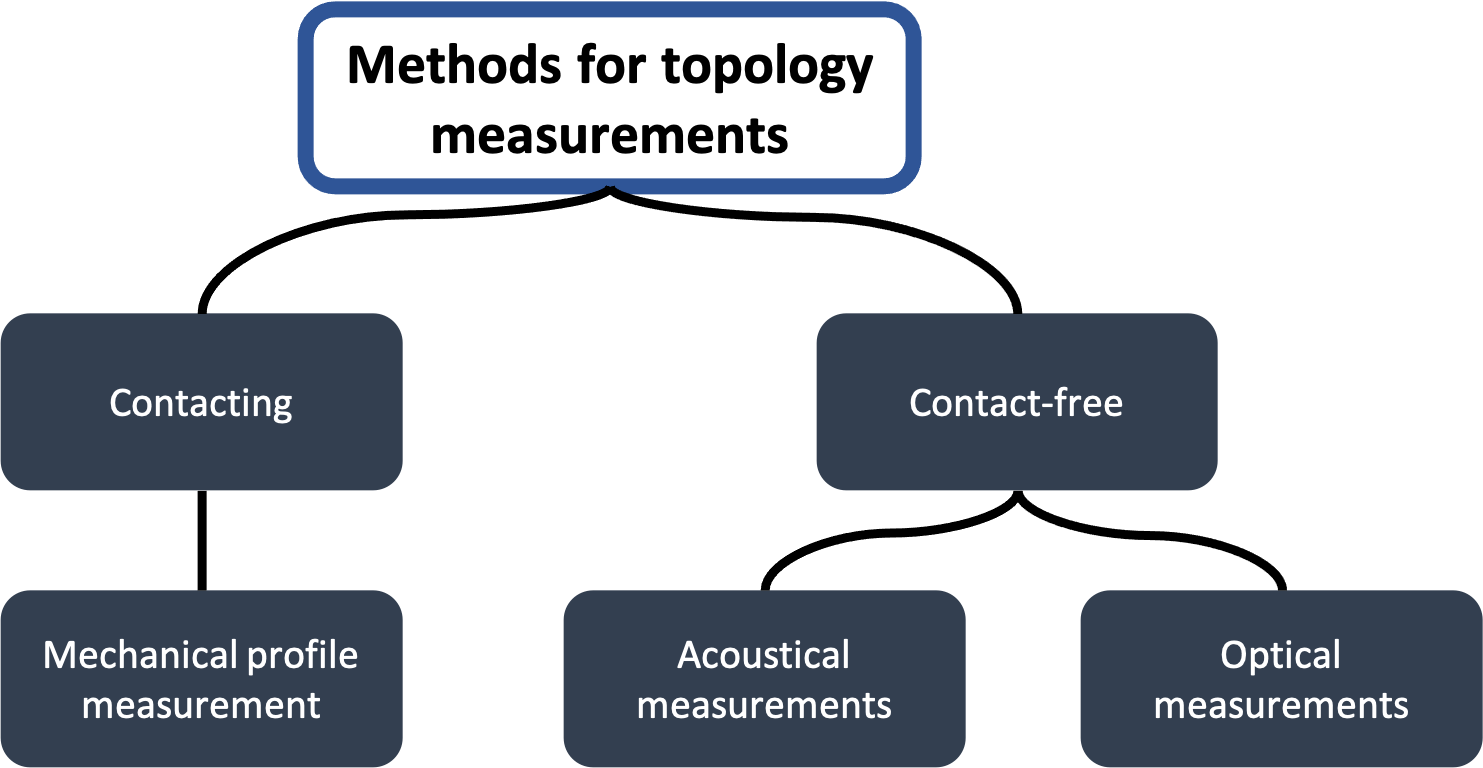
\includegraphics[width=12cm]{Pictures/TopologyMM}
\caption[Diagram of the different types of topology measurements]{Diagram of the different types of topology measurements\cite{Lake2016}}
\label{TopologyMM}
\end{center}
\end{figure}

\subsubsection{Profilometry}
One of the most common mechanical surface measurement methods is performed with a measurement device called "Profilometer". This measurement instrument drags a small diamond or ruby tipped stylus across the surface of the sample. The stylus is mounted in a way that allows the tip to move up and down according to the surface topography of the sample. This motion is then converted into an electrical signal, which gets amplified and digitised in order to image the surface profile. The advantage of a profilometer is that they are relatively inexpensive, simple to use and connected to valid standards in research and industry. One of the big disadvantages of such a device is the mechanical interaction between the tip of the stencil and the sample. The diamond tip can leave scratch marks on hard surfaces or deform soft surfaces what ultimately leads to bad measurement results. Another limitation of a profilometer is, as the name suggests, that it can only pick up the profile of a surface on a specific point/line. This makes it easy to miss local imperfections.\cite{Rebeggiani2009}\cite{Lake2016}

\subsubsection{Interferometry}
Interferometry is a very sensitive optical measurement technique used in a wide variety of metrology applications. It is based on the principle of interference between electromagnetic waves. The most basic setup of an interferometer is the "Michelson Interferometer" (see figure \ref{Interferometer}). In the Michelson interferometer a laser beam is sent into a beamsplitter, which splits the laser beam and directs it towards two reflectors. Usually one of these reflectors is used as a reference and fixed in space. The other one can be moved closer or further away. Both of the from the reflectors returned laser beams are now superimposed onto a detecter, where they create an interference pattern. The interference pattern will change based on the phase shift between the two light waves. This phase shift is directly dependent on the position of the movable reflector. That said, it is important to note, that this is a relative measurement. The position of the movable reflector can only be calculated relative to its initial position as a multiple of the wavelength of the used laser. Depending on the used detector, an interferometric measurement setup can reach sub-nanometer precision.\\
For surface metrology, an interferometer is used to precisely image the surface of a sample. It has the big advantage, that it can pick up a surface contact free. This lowers the chance of missing features of a surface when compared to a profiling measurement technique. In figure \ref{Interferometer} an example of surface measurement with a so called white light interferometer is shown.


\begin{figure}
\begin{center}
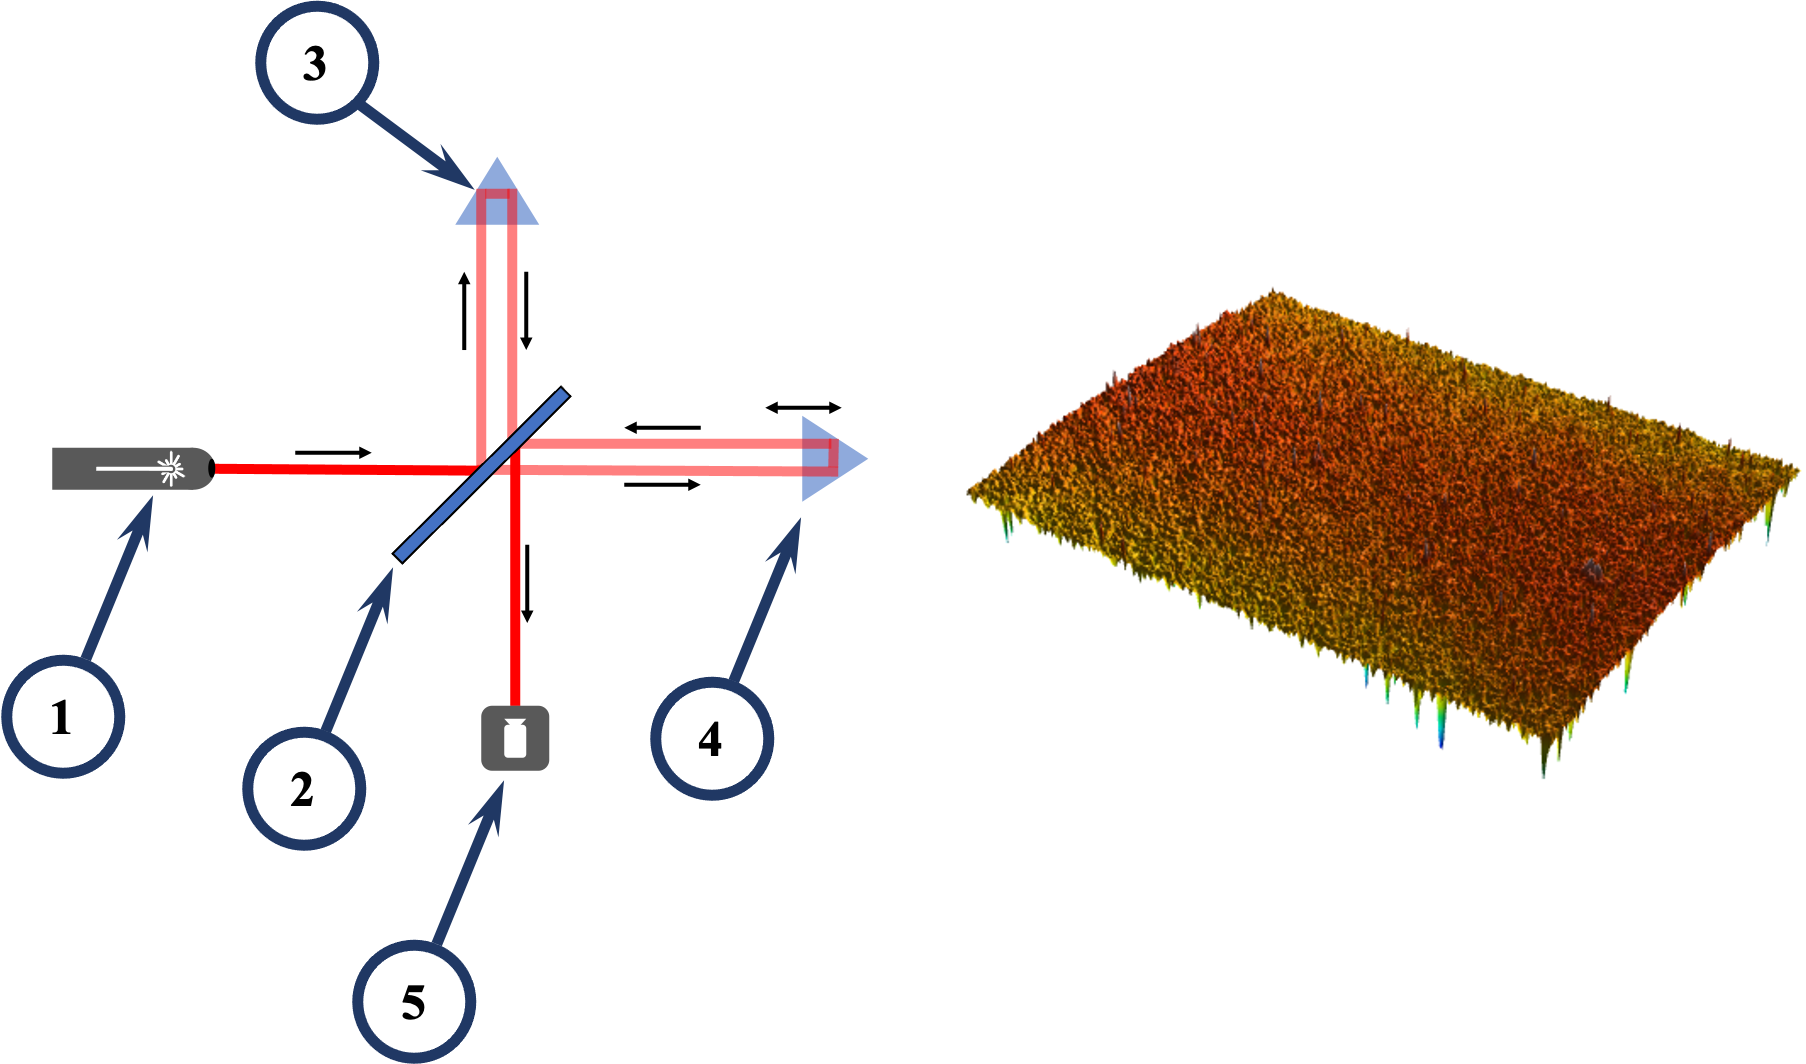
\includegraphics[width=12cm]{Pictures/Interferometer}
\caption[Schematic of an Michelson interferometer setup]{Schematic of an Michelson interferometer setup: Left - Michelson interferometric setup, Right - Interferometer measurement of a chrome surface, 1 - Laser source, 2 - Beamsplitter, 3 - Reference mirror, 4 - Movable mirror, 5 - Detector (camera)}
\label{Interferometer}
\end{center}
\end{figure}











\section{Data acquisition and processing}
\subsection{MATLAB}
\textbf{MAT}rix \textbf{LAB}oratory (MATLAB) is an \textbf{I}ntegrated \textbf{D}evelopment \textbf{E}nvironment (IDE) and programming language. MATLAB was developed in the need of a numerical algebraic system at the university of New Mexico. On this base, the company MathWorks (see Appendix \ref{AppLoC}) was created. Since 1984 MathWorks is further developing MATLAB and additional software for numerical algebraic computing. To support different hardware packages MathWorks offers so called toolboxes. These toolboxes contain functions and scripts for communication, data acquisition, motion control etc.\cite{Mathworks}\\
MATLAB is mainly used in technical development and research. During this project it was used for data analysis.

\subsection{LabVIEW}
\textbf{Lab}oratory \textbf{V}irtual \textbf{I}nstrument \textbf{E}ngineering \textbf{W}orkbench (LabVIEW) is a cross platform development environment for the graphical programming language called "G" developed by National Instruments (see Appendix \ref{AppLoC}). LabVIEW offers an easy way to design graphical user interfaces (GUI) by coupling the logical code with a "Frontpanel" which contains Indicators and Dials for the user to interact with. Both, G and LabVIEW, are focused on fast data acquisition and analysis using parallel computing (multi threading). Aimed towards laboratory environments, LabVIEW offers support for a wider variety of hardware, such as Thorlabs or National Instruments' own data acquisition and test hardware.\cite{whatisLabVIEW}\\
During this project LabVIEW was used for data acquisition and analysis. Further the GUI to control the Artificial Eye was created using LabVIEW.

















